\section{Begrüßung}

\begin{spacing}{1.5}
    \setlength{\parskip}{1.6ex}

    Hallo liebe Erstis,

    wir, der Fachschaftsrat, oder auch kurz FSR, 
    begrüßen euch ganz herzlich an der MLU.
    Mit unseren pinken T-Shirts sind wir den meisten 
    von euch ja schon bei den Erstiveranstaltungen begegnet.
    Neben der Erstiwoche sorgen wir während eurer gesamten Studienzeit
    für ein bisschen Spaß neben dem Alltagstrott, 
    stehen euch aber auch bei jeglichen Fragen zur Seite.
    Achtet im Institut auf unsere Plakate für Spieleabende und die Weihnachtsfeier.
    Wir freuen uns, wenn ihr vorbei kommt!

    Als frisch gebackene Studierende seid ihr sicher gespannt, 
    was euch in den nächsten Monaten 
    an der Universität erwarten wird. 
    In den nächsten Wochen werdet ihr, 
    neben der ein oder anderen Ersti-Party,
    auch die ersten Vorlesungen und Übungen besuchen.

    Ganz schön viel Neues -- 
    aber zusammen mit euren Kommilitonen 
    lassen sich die Übungsserien viel leichter stemmen.
    Und aus den anfänglichen Lerngruppen 
    können im Laufe der Zeit schnell Freunde fürs Leben werden.
    Ihr kommt mit den Übungen nicht klar? 
    Kommt mal in den Tutorien, 
    oder im Mathe-~oder Info-Treff vorbei, 
    wo euch andere Studierende bei den Aufgaben unterstützen.

    Auch wenn wegen Corona immer noch alles ein bisschen anders läuft,
    versuchen wir und eure Institute, euch den Start ins Studium 
    so einfach wie möglich zu machen. Falls das mal nicht funktioniert, wendet euch an uns.

    Wir wünschen euch viel Spaß und Erfolg im Studium!

    Euer Fachschaftsrat \\
    \email{fachschaft@mathinf.uni-halle.de}
\end{spacing}
\vspace*{-1ex}
\begin{center}
    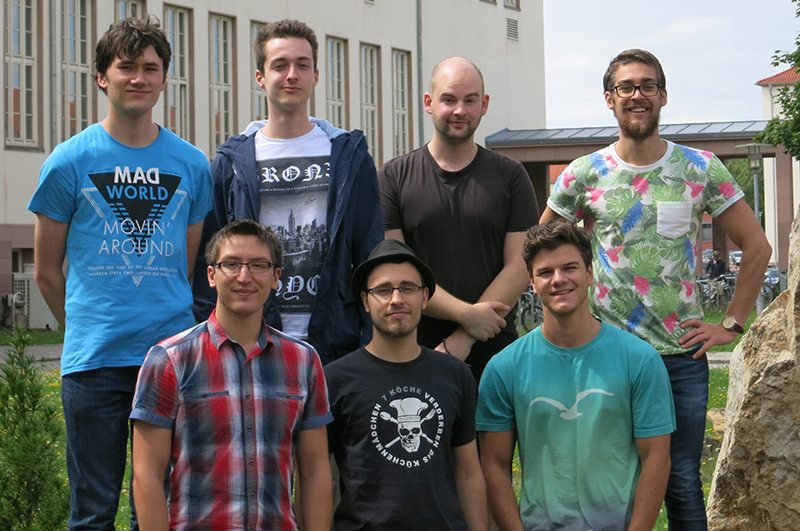
\includegraphics[width=1\linewidth]{fsr}
\end{center}%
FSR (v.l.n.r.): 
Jan Heinrich Reimer,
Jonas Findeisen,
Henrike Schweizer,
Anouk Ronja Océane Duyster,
Anna Iudaeva,
Aaron Gröbel, 
Patrick Tischendorf,
Fabian Kiesner.
Sonne:
Lenz Hank-Weise.

